\documentclass[../main.tex]{subfiles}
\graphicspath{{\subfix{../images/}}}
\usepackage{amsmath}
\usepackage{tikz}
\usepackage{pgfplots}
\usetikzlibrary{patterns}
\pgfplotsset{compat=1.18}
\newcommand{\un}[1]{\underline{#1}}
\newcommand{\partFrac}[2]{\frac{\partial #1}{\partial #2}}
\begin{document}
	\paragraph{Calculate Divergance Theorem}
		Given the vector field, where $z=0$:
		\begin{equation}
			\underline{v}=3y^{2}z\underline{i} + 2y^{2}\underline{j} + yz^{2}\underline{k}
		\end{equation}
		\begin{equation}
			\underline{v} = 2y^{2}\underline{j}
		\end{equation}
		The divergance theorem is given by:
		\begin{equation*}
			\iint_A \nabla \cdot \underline{v} dA  = \oint \underline{n} \cdot \underline{v} dr
		\end{equation*}
		Calculating the inside of the LHS:
		\begin{equation*}
			\nabla \cdot \un{v} = \un{j} \partFrac{}{y} \cdot 2y^{2} \un{j} = 4y
		\end{equation*}
		Therefor calculating LHS:
		\begin{equation*}
			\iint_A \nabla \cdot \underline{v} \; dA  = \int_{2}^{3} \int_2^4 4y \;dxdy
		\end{equation*}
		\begin{equation*}
			\iint_A \nabla \cdot \underline{v} \; dA  = \Big| 8 \frac{y^2}{2} \Big|_2^3 = 20
		\end{equation*}

		Calculating the RHS, using the graphic finding the normal vectors to each side. Only two terms
		are present as i dot j will be zero, so the verticals are zero.

		\begin{equation*}
			\oint \underline{n} \cdot \underline{v} dr = \int_2^4 -\un{j} \cdot 2y^2\un{j} dx + \int_2^4 \un{j} \cdot 2y^2\un{j} dx 
		\end{equation*}
		Using Figure:\ref{fg:1} replacing the y values from the graphic, 2 and 3 respectivly
		\begin{equation*}
			= \int_2^4 -8 dx + \int_2^4 18 dx = 20
		\end{equation*}
		Therefor RHS = LHS
		\begin{figure}[ht]
			\centering
			\caption{Vector Field Figure}
			\label{fg:1}
			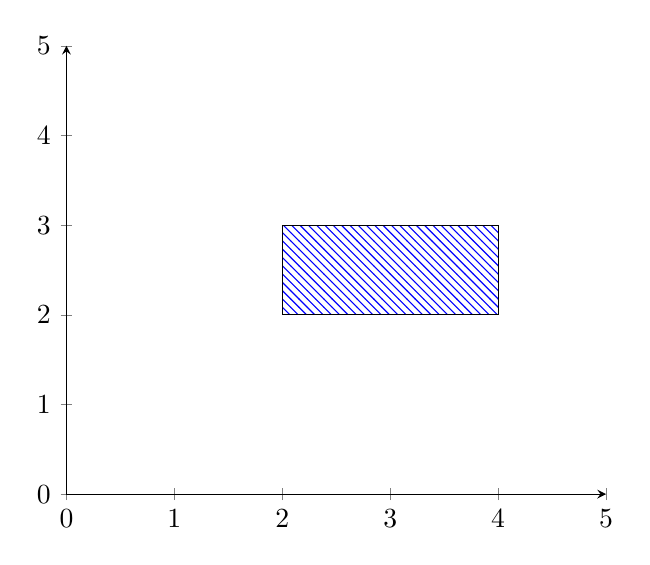
\begin{tikzpicture}
			\begin{axis}[xmin=0, xmax=5, ymin=0, ymax=5, axis x line=bottom, axis y line=left]
				\draw[pattern=north west lines, pattern color=blue] (2,2) rectangle (4,3);
			\end{axis}
			\end{tikzpicture}
		\end{figure}


	\paragraph{Calculate Stokes Integral Theorem} for the velocity field $v=x \un{j}$.
		\\ Stokes integral is given by:
		\begin{equation*}
			\oint_{\partial S} \un{v}\cdot dr = \iint_S \un{n} \cdot \nabla \times \un{v} \; dS
		\end{equation*}
		Calculating the LHS:
		\begin{align*}
			\oint_{\partial S} \un{v}\cdot dr &= \int (x\un{j}) \cdot (dx \cdot \un{i} + dy \cdot \un{j}) \\
											  &= \int x dy
		\end{align*}
		The only non zero term is in the vertical because the dot product is 0 for non-equal unit vectors 
		\footnote{Split integrals if more than one direction in velocity field}
		\\ Based on Figure: \ref{fg:2} respect the rotations when picking the bounds for the integrals:
		\begin{align*}
			LHS &= \int_2^3 x dy + \int_3^2 x dy \\
				&= \int_2^3 4 dy + \int_3^2 2 dy \\
				&= 2
		\end{align*}

		Calculating the RHS:
		The normal vector using the right hand rule, based on the rotation is $\un{k}$
		\begin{align*}
			\iint_S \un{n} \cdot \nabla \times \un{v} \; dS &= \iint \un{k} \cdot \un{k} \; dS \\
															&= \int_2^3 \int_2^4 dxdy \\
															&= 2
		\end{align*}
		The inside cross product between the Del and V:
		\begin{equation*}
			\nabla \times \un{v} = \un{i} \partFrac{}{x} \times (x \un{j}) = \un{k}
		\end{equation*}
		The partial cancels the x term and i cross j by convention is k. Only the x partial is included as all the 
		other partials would be zero. \\
		Therefor LHS = RHS \\
		\\
		Figure \ref{fg:2}, has arrows indicating the force and magnitude of different positions, they indicate that the rotation is
		anti-clockwise
		\begin{figure}[ht]
			\centering
			\caption{Stokes Integral Figure}
			\label{fg:2}
			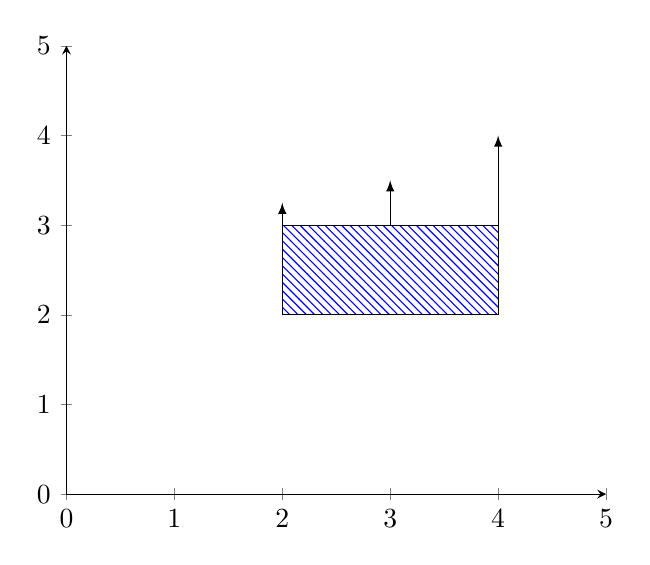
\begin{tikzpicture}
			\begin{axis}[xmin=0, xmax=5, ymin=0, ymax=5, axis x line=bottom, axis y line=left]
				\draw[pattern=north west lines, pattern color=blue] (2,2) rectangle (4,3);
				\draw [-latex](4,3) -- (4,4);
				\draw [-latex](3,3) -- (3,3.5);
				\draw [-latex](2,3) -- (2,3.25);
			\end{axis}
			\end{tikzpicture}
		\end{figure}
\end{document}
